5. \begin{figure}[ht!]
\center{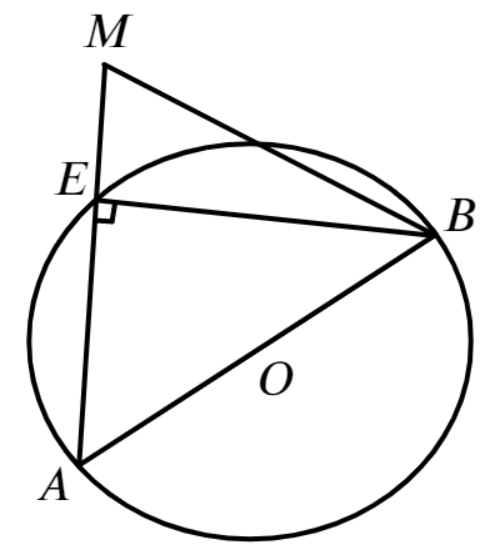
\includegraphics[scale=0.35]{g8-5.png}}
\end{figure}\\
В прямоугольном треугольнике медиана, проведённая из прямого угла, равна половине гипотенузы, значит $AB=2CM=24$см. Проведём высоту $CD,$ треугольники $ANH$ и $ACD$ подобны по двум углам (один прямой и один общий), значит $\cfrac{CD}{NH}=\cfrac{AC}{AN}=2,$ откуда $CD=2\cdot3=6$см. Тогда $S_{\Delta ABC}=\cfrac{1}{2} CD\cdot AB=\cfrac{1}{2}\cdot6\cdot24=72\text{ см}^2.$\\
